% This file was created by tikzplotlib v0.9.8.
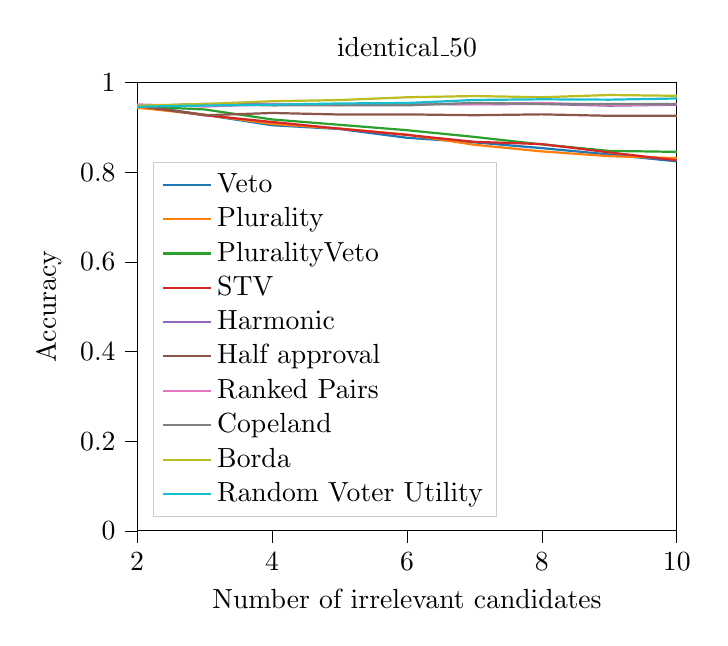
\begin{tikzpicture}

\definecolor{color0}{rgb}{0.12156862745098,0.466666666666667,0.705882352941177}
\definecolor{color1}{rgb}{1,0.498039215686275,0.0549019607843137}
\definecolor{color2}{rgb}{0.172549019607843,0.627450980392157,0.172549019607843}
\definecolor{color3}{rgb}{0.83921568627451,0.152941176470588,0.156862745098039}
\definecolor{color4}{rgb}{0.580392156862745,0.403921568627451,0.741176470588235}
\definecolor{color5}{rgb}{0.549019607843137,0.337254901960784,0.294117647058824}
\definecolor{color6}{rgb}{0.890196078431372,0.466666666666667,0.76078431372549}
\definecolor{color7}{rgb}{0.737254901960784,0.741176470588235,0.133333333333333}
\definecolor{color8}{rgb}{0.0901960784313725,0.745098039215686,0.811764705882353}

\begin{axis}[
legend cell align={left},
legend style={
  fill opacity=0.8,
  draw opacity=1,
  text opacity=1,
  at={(0.03,0.03)},
  anchor=south west,
  draw=white!80!black
},
tick align=outside,
tick pos=left,
title={identical\_50},
x grid style={white!69.0196078431373!black},
xlabel={Number of irrelevant candidates},
xmin=2, xmax=10,
xtick style={color=black},
y grid style={white!69.0196078431373!black},
ylabel={Accuracy},
ymin=0, ymax=1,
ytick style={color=black}
]
\addplot [thick, color0]
table {%
2 0.9493
3 0.928
4 0.9047
5 0.8963
6 0.8767
7 0.8665
8 0.8536
9 0.8394
10 0.8241
};
\addlegendentry{Veto}
\addplot [thick, color1]
table {%
2 0.9438
3 0.9282
4 0.9077
5 0.8972
6 0.8839
7 0.8611
8 0.8463
9 0.8356
10 0.8312
};
\addlegendentry{Plurality}
\addplot [thick, color2]
table {%
2 0.9467
3 0.9399
4 0.9176
5 0.9056
6 0.8936
7 0.8786
8 0.8619
9 0.8474
10 0.8453
};
\addlegendentry{PluralityVeto}
\addplot [thick, color3]
table {%
2 0.9489
3 0.9272
4 0.9119
5 0.8971
6 0.883
7 0.8677
8 0.8626
9 0.8441
10 0.8264
};
\addlegendentry{STV}
\addplot [thick, color4]
table {%
2 0.9464
3 0.9523
4 0.952
5 0.9506
6 0.9524
7 0.9512
8 0.9522
9 0.9482
10 0.9504
};
\addlegendentry{Harmonic}
\addplot [thick, color5]
table {%
2 0.9476
3 0.9269
4 0.932
5 0.9286
6 0.9288
7 0.927
8 0.9289
9 0.9257
10 0.9257
};
\addlegendentry{Half approval}
\addplot [thick, color6]
table {%
2 0.9511
3 0.9463
4 0.9512
5 0.9499
6 0.9514
7 0.9523
8 0.9543
9 0.9496
10 0.9515
};
\addlegendentry{Ranked Pairs}
\addplot [thick, white!49.8039215686275!black]
table {%
2 0.9471
3 0.9519
4 0.9489
5 0.9491
6 0.949
7 0.9545
8 0.9522
9 0.9522
10 0.952
};
\addlegendentry{Copeland}
\addplot [thick, color7]
table {%
2 0.9483
3 0.9521
4 0.9582
5 0.9608
6 0.967
7 0.9698
8 0.9671
9 0.9721
10 0.9703
};
\addlegendentry{Borda}
\addplot [thick, color8]
table {%
2 0.9459
3 0.9486
4 0.9505
5 0.9532
6 0.9542
7 0.961
8 0.9625
9 0.9617
10 0.9643
};
\addlegendentry{Random Voter Utility}
\end{axis}

\end{tikzpicture}
